\documentclass[11pt]{article}
\usepackage[margin=0.75in]{geometry}
\usepackage{amsmath}
\usepackage{tikz}
\usepackage{enumitem}
\usepackage{siunitx}
\setlength{\parindent}{0pt}
\newcommand{\graphbox}{\begin{center}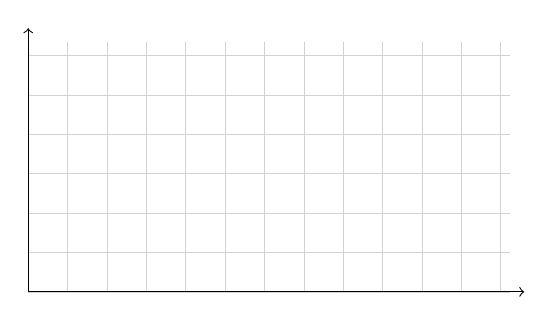
\begin{tikzpicture}[x=0.72cm,y=0.72cm]
\draw[step=0.5cm,gray!35,very thin] (0,0) grid (8.5,4.4);
\draw[->] (0,0)--(8.75,0); \draw[->] (0,0)--(0,4.65);
\end{tikzpicture}\end{center}}
\begin{document}
\begin{center}\Large\textbf{AP Physics 1 1D Motion Post-Lab Quiz -- Version D}\end{center}
\vspace{0.08in}\textbf{Name:} \rule{2.1in}{0.4pt}\hfill\textbf{Period:} \rule{0.65in}{0.4pt}\hfill\textbf{Date:} \rule{1.1in}{0.4pt}
\vspace{0.12in}
\begin{enumerate}[leftmargin=*,itemsep=0.15in]
\item A student drops a ball from rest from a fixed height and records only the total time between releasing the ball and the ball reaching the floor.

\textbf{a.} Explain why this single measurement is not enough to determine how the ball's speed changes during the fall.\\
\textbf{b.} Identify an additional set of measurements that would allow the student to better analyze the motion.
\vspace{0.55in}

\item A student releases a ball from rest and records its position at only three different times during the fall. The student considers repeating the experiment while recording the ball's position at eight different times instead.

\textbf{a.} Explain why collecting more position-time data points could improve the analysis.\\
\textbf{b.} Identify one condition that should remain unchanged when the student collects the additional measurements.
\vspace{0.55in}

\item A student releases a ball from rest and measures how far it has fallen.

\begin{center}
\begin{tabular}{c|cccccc}
Time $t$ (s) & 0.00 & 0.10 & 0.20 & 0.30 & 0.40 & 0.50\\ \hline
Distance fallen $d$ (m) & 0.000 & 0.049 & 0.195 & 0.442 & 0.781 & 1.227
\end{tabular}
\end{center}
\textbf{a.} Transform the data as needed to produce a linear graph. Using the graph space provided, plot the appropriate variables, clearly label both axes with units, and draw a best-fit line.\\
\textbf{b.} Describe the shape of your graph. Based on the graph, determine whether the ball's acceleration was approximately constant and explain your reasoning.

\graphbox
\end{enumerate}
\end{document}
